\section{Realization}
%Focus generale sulle tecnologie utilizzate
In this section we outline the technical aspects concerning the realization of our framework. Therefore we first present the enabler technologies through which we instantiate the design principles presented in \cref{sec:design}. After that, we discuss the interaction workflow between the instantiated technologies. Finally, we show the implementation details.
\begin{figure}[t]
\centering
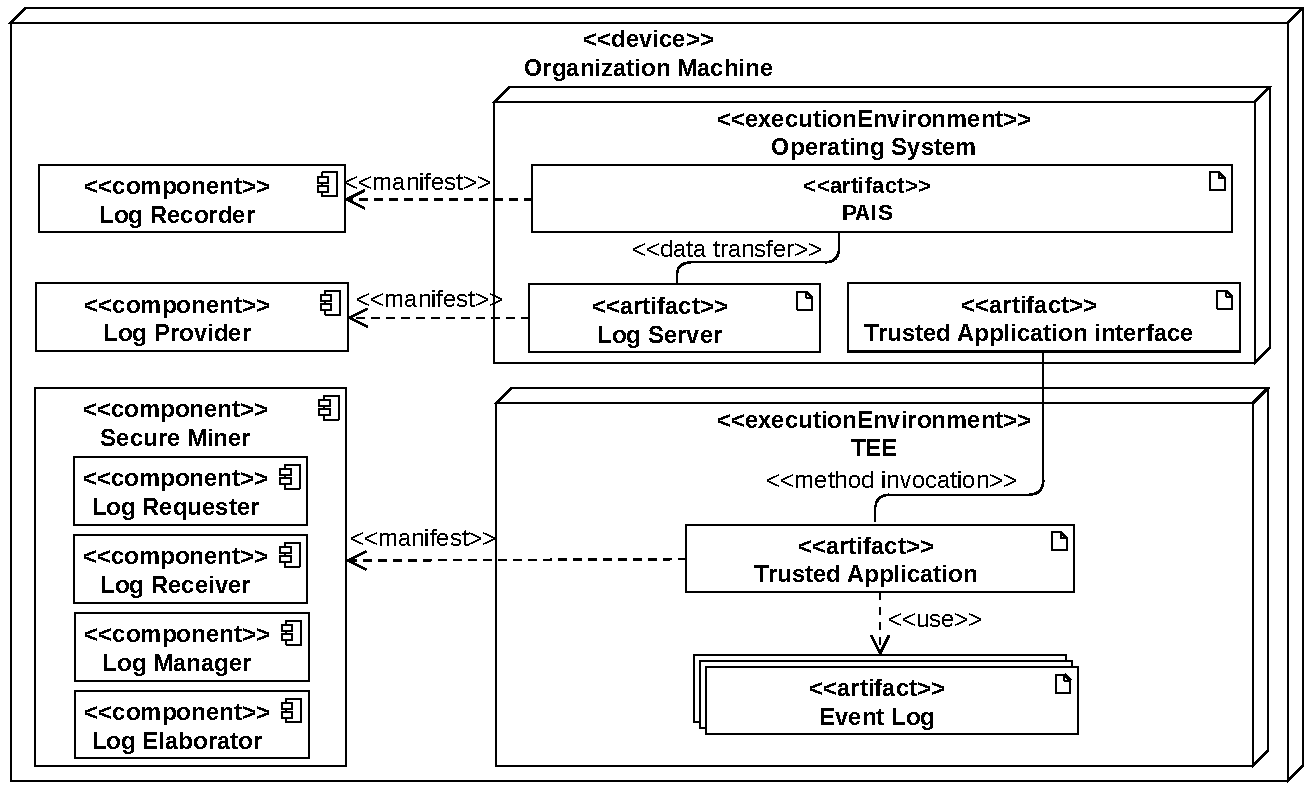
\includegraphics[width=11cm]{content/figures/deployment_diagram.pdf}
\caption{UML deployment diagram.}
\label{fig:deployment_diagram}
\end{figure}
\subsection{Deployment}
As follow, we bridge the gap between high-level system architecture and its practical realization. \cref{fig:deployment_diagram} depicts a \textit{UML deployment diagram} \cite{koch2002expressive} aimed at aiding the understanding of the instantiated infrastrucuture. 

The \texttt{Organization Machine} represent the physical computation \textit{device} embracing the software and hardware entities of the company. The \texttt{PAIS}, the \texttt{PAIS Interface}, the \texttt{Log Provider} and \texttt{Secure Miner} are included in the \texttt{Organization Machine} as abstract \textit{components} . These elements serve as logical containers that incorporate the core functionalities already discussed in \cref{sec:design}. The \texttt{Organization Machine} is characterized by two \textit{execution environment}s: The \texttt{Operative System} and the \texttt{Trusted Execution Environment}.

\subsection{Workflow}
\subsection{Implementation}
%\subsubsection{Event Log Generation}
%Tecnologie utilizzate
%Sintesi del processo di generazione dei log
%\subsubsection{Trusted Miner and Log Provider}
%Tecnologia TEE usata
%Linguaggio usato per programmare in TEE
%Algoritmo implementato
%Rappresentazioni intermedie (PNML, Petrinet, ecc...)
%Linguaggio Log provider
